\section{反射型フォトセンサの理論式}
\begin{figure}[H]
\begin{center}
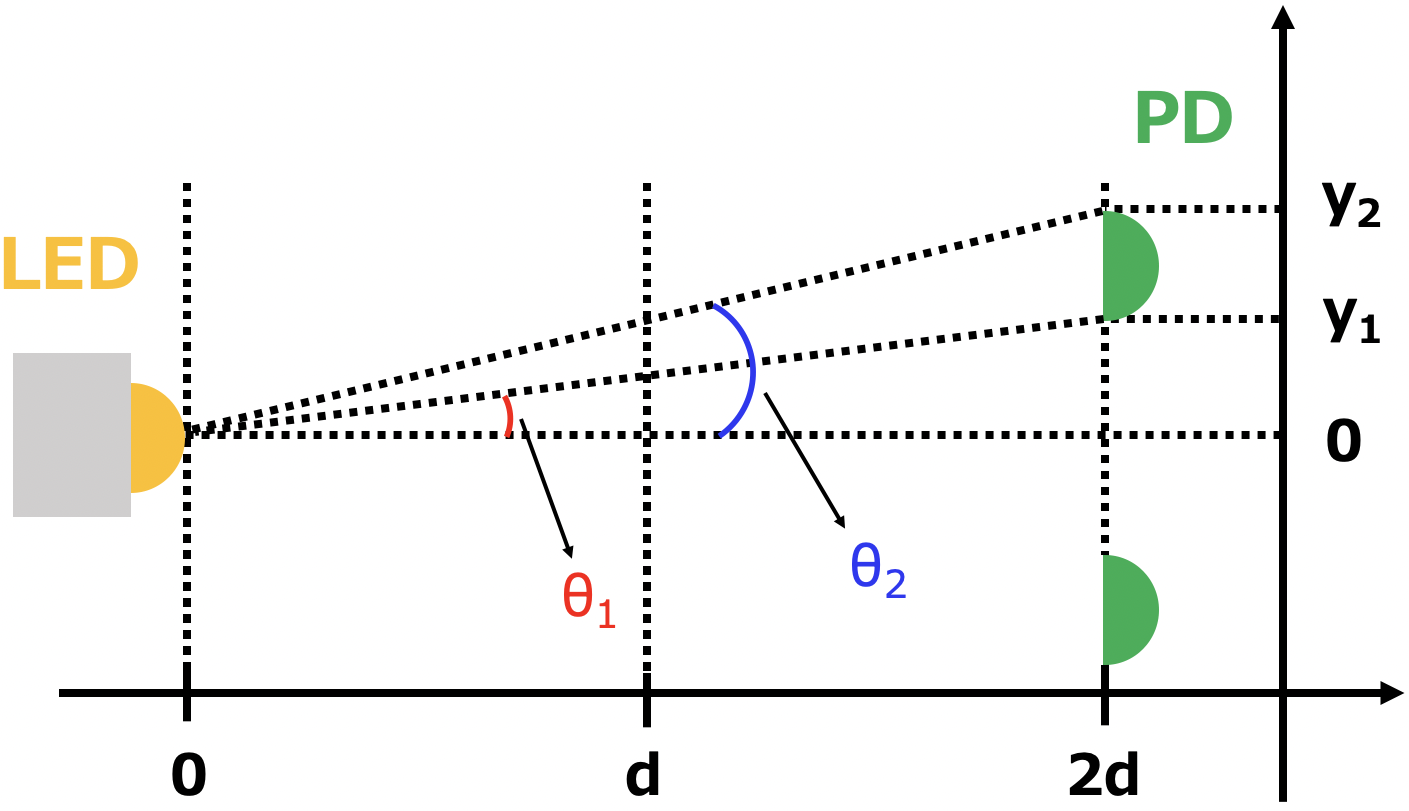
\includegraphics[width=140mm]{figC_1.png}
\caption[反射型フォトセンサの2次元モデル]{反射型フォトセンサの2次元モデル}
\label{figC.1}
\end{center}
\end{figure}
\ref{sec4.2.2.2}節で記した通り, KAGRAではダンピング制御に用いるセンサとして, 反射型フォトセンサを用いている. ここでは反射型フォトセンサの応答について, 図\ref{figC.1}に示したような2次元応答モデルを考え, その理論式を示す. \\
\quad 反射型フォトセンサの動作原理は図\ref{fig4.13}に示す通り, LEDから出た光が距離$d$だけ離れたターゲット(懸架装置の各ステージ)で反射してLEDと同じ位置にあるPDに帰ってくる光量の変化を読み取るというものである. よってLEDから出た後PDに入るまでに光は水平距離(図C.1の横軸方向)で2d進むことになる. そこで, ここではLEDから出た光がターゲットで$n$回反射して, 2$d$の距離だけ離れたPDに入るという状況を考える. \\
\quad さらにPDの各端の位置を図\ref{figC.1}のようにそれぞれ$y_1,\,\,y_2$とし, そこに向かう角度を$\theta_1,\,\,\theta_2$とすると
\begin{equation}
y_1=2nd\times\tan\theta_1,
\label{eqC.1}
\end{equation}
\begin{equation}
y_2=2nd\times\tan\theta_2.
\label{eqC.2}
\end{equation}
ここで, LEDの光は直進性が強く, 配光角(明るく照らすことのできる角度)が限られているため, そのビームプロファイルは角度に依存すると考え, $I(\theta)$と書く. このとき, PDが対称に2つ取り付けられていることに注意すると, 反射型フォトセンサの出力応答は
\begin{equation}
O(d)=2\sum\limits_{n}r^n\int_{\theta_1}^{\theta_2}I(\theta){\rm d}\theta.
\end{equation}
ただし, $r$は光の反射率を表す. この式と式(\ref{eqC.1}), (\ref{eqC.2})を合わせて反射型フォトセンサの出力を求めることができる. \\
\quad さて, 光がガウシアンビームだとすると
\begin{equation}
I(\theta)=\frac{1}{\sqrt{\pi\sigma^2}}{\rm e}^{-\frac{(x-\mu)^2}{2\sigma^2}},
\end{equation}
と書ける. また, KAGRAで用いられている反射型フォトセンサは$y_1=8$ mm, $y_2=10$ mmである\cite{47}. この値を用いてその応答をプロットすると, 図\ref{figC.2}のようになる. \\
\quad 図を見ると, 距離が離れるにしたがって低次の反射光がPDに入るようになるとセンサの応答は大きくなっている. これは低次の反射光は高次のものに比べて光量が多いためである. その後, 1次の反射光の広がりがPDをカバーするようになると, 距離の増加に伴って光量が減少し, 出力は小さくなっていく. 
\quad なお, 赤線がガウシアンアンビーム, 青線が等方的に広がるビームの場合である. ガウシアンビームの場合, ビーム幅が広く, ピーク以降も強い光の高次反射光(ビーム中心)がPDに入る. よって, 等方的な場合に比べ, ピーク付近の応答が緩やかであり, 線形範囲が広くなっている. また, これより低温懸架装置で用いられる反射型フォトセンサでは, およそ$10\,\,{\rm mm}\sim35\,\,{\rm mm}$の距離測定
で使うことができる.
\begin{figure}[H]
\begin{center}
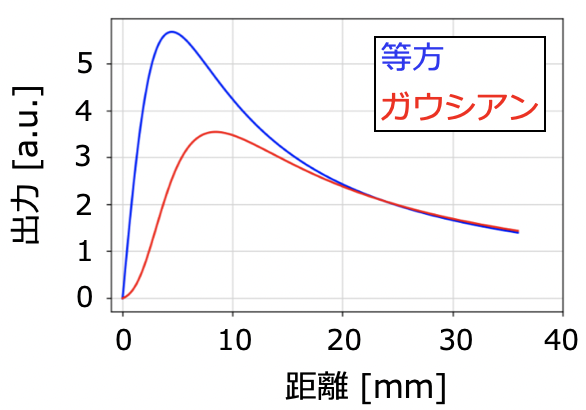
\includegraphics[width=120mm]{figC_2.png}
\caption[反射型フォトセンサの応答]{反射型フォトセンサの応答. 低次の反射光がPDに入るようになるとセンサの応答は大きくなり, その後は距離の増加に伴って光量が減少するので出力は小さくなっていく. また, ガウシアンビームはビーム幅が広く, 等方的なビームに比べて線形範囲が広い. }
\label{figC.2}
\end{center}
\end{figure}